%%%%%%%%%%%%%%%%%%%%%%%%%%%%%%% beamer %%%%%%%%%%%%%%%%%%%%%%%%%%%%%%%%%%%%%%%%%%%%%%%%%
% To run - pdflatex filename.tex
%	   acroread filename.pdf
%%%%%%%%%%%%%%%%%%%%%%%%%%%%%%%%%%%%%%%%%%%%%%%%%%%%%%%%%%%%%%%%%%%%%%%%%%%%%%%%%%%%%%%%
% without pauses
%\documentclass[compress,red, handout]{beamer}
\documentclass[compress, red]{beamer}
\mode<presentation>
\setbeamertemplate{navigation symbols}{}

\usetheme{Warsaw}

% other themes: AnnArbor, Antibes, Bergen, Berkeley, Berlin, Boadilla,
% boxes, CambridgeUS, Copenhagen, Darmstadt, default, Dresden,
% Frankfurt, Goettingen, Hannover, Ilmenau, JuanLesPins, Luebeck,
% Madrid, Maloe, Marburg, Montpellier, PaloAlto, Pittsburg, Rochester,
% Singapore, Szeged, classic

% \usecolortheme{lily} color themes: albatross, beaver, beetle, crane,
% default, dolphin, dov, fly, lily, orchid, rose, seagull, seahorse,
% sidebartab, structure, whale, wolverine

%\usefonttheme{serif}
% font themes: default, professionalfonts, serif, structurebold, structureitalicserif, structuresmallcapsserif

\hypersetup{pdfpagemode=FullScreen} % makes your presentation go automatically to full screen

% define your own colors:
\definecolor{Red}{rgb}{1,0,0}
\definecolor{Blue}{rgb}{0,0,1}
\definecolor{Green}{rgb}{0,1,0}
\definecolor{magenta}{rgb}{1,0,.6}
\definecolor{lightblue}{rgb}{0,.5,1}
\definecolor{lightpurple}{rgb}{.6,.4,1}
\definecolor{gold}{rgb}{.6,.5,0}
\definecolor{orange}{rgb}{1,0.4,0}
\definecolor{hotpink}{rgb}{1,0,0.5}
\definecolor{newcolor2}{rgb}{.5,.3,.5}
\definecolor{newcolor}{rgb}{0,.3,1}
\definecolor{newcolor3}{rgb}{1,0,.35}
\definecolor{darkgreen1}{rgb}{0, .35, 0}
\definecolor{darkgreen}{rgb}{0, .6, 0}
\definecolor{darkred}{rgb}{.75,0,0}

\xdefinecolor{olive}{cmyk}{0.64,0,0.95,0.4}
\xdefinecolor{purpleish}{cmyk}{0.75,0.75,0,0}

% can also choose different themes for the "inside" and "outside"

% \usepackage{beamerinnertheme_______}
% inner themes include circles, default, inmargin, rectangles, rounded

% \usepackage{beamerouterthemesmoothbars} outer themes include
% default, infolines, miniframes, shadow, sidebar, smoothbars,
% smoothtree, split, tree


% to have the same footer on all slides
%\setbeamertemplate{footline}[text line]{STUFF HERE!}
%\setbeamertemplate{footline}[text line]{} % makes the footer EMPTY

%To generate note pages after each slide
%\setbeameroption{show notes}

% include packages
\usepackage{subfigure}
\usepackage{multicol}
\usepackage{amsmath}
\usepackage{epsfig}
\usepackage{graphicx}
\usepackage[all,knot]{xy}
\xyoption{arc}
\usepackage{url}
\usepackage{multimedia}
\usepackage{hyperref}
\usepackage{helvet}
\usepackage[polish,english]{babel}
\usepackage[utf8]{inputenc}
\usepackage{textcomp} % for \textmu (greek letter mu without the need
                      % to use Math mode)
     
%%%%%%%%%%%%%%%%%%%%%%%%%%%%%%%%%%%%%%%%%%%%%%%%%%%%%%%%%%%%%%%%%%%%%%%%%%%%%%%%%%%%%%%%%%
%%%%%%%%%%%%%%%%%%%%%%%%%%%%%% Title Page Info %%%%%%%%%%%%%%%%%%%%%%%%%%%%%%%%%%%%%%%%%%%
%%%%%%%%%%%%%%%%%%%%%%%%%%%%%%%%%%%%%%%%%%%%%%%%%%%%%%%%%%%%%%%%%%%%%%%%%%%%%%%%%%%%%%%%%%

\title{White Rabbit}
%\subtitle{A short introduction}
\author[J. Serrano] % (optional, use only with lots of authors)
{Javier Serrano}
\institute{CERN BE-CO\\Hardware and Timing section}
\date[1 July 2014]{European Frequency and Time Seminar\\Besançon, 1 July 2014}

\AtBeginSection[]
{
  \begin{frame}<beamer>{Outline}
    \tableofcontents[currentsection]
  \end{frame}
}

%%%%%%%%%%%%%%%%%%%%%%%%%%%%%%%%%%%%%%%%%%%%%%%%%%%%%%%%%%%%%%%%%%%%%%%%%%%%%%%%%%%%%%%%%%
%%%%%%%%%%%%%%%%%%%%%%%%%%%%%% Begin Your Document %%%%%%%%%%%%%%%%%%%%%%%%%%%%%%%%%%%%%%%
%%%%%%%%%%%%%%%%%%%%%%%%%%%%%%%%%%%%%%%%%%%%%%%%%%%%%%%%%%%%%%%%%%%%%%%%%%%%%%%%%%%%%%%%%%
\useoutertheme[subsection=false]{smoothbars}
%\setbeamertemplate{footline}[frame number]


\begin{document}

%%%%%%%%%%%%%%%%%%%%%%%%%%%%%%%%%%%%%%%%%%%%%%%%%%%%%%%%%%%%%%%%%%%%%%%%%%%%%%%%%%%%%%%%%%

\frame{
	\titlepage 
%\hfill {\footnotesize With help from Steve Smith (SLAC)}
}

%%%%%%%%%%%%%%%%%%%%%%%%%%%%%%%%%%%%%%%%%%%%%%%%%%%%%%%%%%%%%%%%%%%%%%%%%%%%%%%%%%%%%%%%%%

% \section[Outline]{} 
% this puts the outline before EACH section automatically & will
% highlight the section you're about to talk about

\frame{\tableofcontents}

% Structuring a talk is a difficult task and the following structure
% may not be suitable. Here are some rules that apply for this
% solution: 

% - Exactly two or three sections (other than the summary).
% - At *most* three subsections per section.
% - Talk about 30s to 2min per frame. So there should be between about
%   15 and 30 frames, all told.

% - A conference audience is likely to know very little of what you
%   are going to talk about. So *simplify*!
% - In a 20min talk, getting the main ideas across is hard
%   enough. Leave out details, even if it means being less precise than
%   you think necessary.
% - If you omit details that are vital to the proof/implementation,
%   just say so once. Everybody will be happy with that.

\section[OSHW Intro]{Introduction to Open Hardware}
\subsection{}
%=======================

\begin{frame}{There is an OSHW definition!}

\begin{block}{Check out \href{http://www.oshwa.org/definition/}{http://www.oshwa.org/definition/}}
\begin{itemize}
 \item Inspired by the Open Source definition for software.
 \item Focuses on ensuring freedom to study, modify, distribute, make
   and sell designs or hardware based on those designs.
 \item Now we know exactly what we mean when we say OSHW!
\end{itemize}
\end{block}
\end{frame}

\begin{frame}{Dispelling the commercial vs open myth}
 \begin{center}
   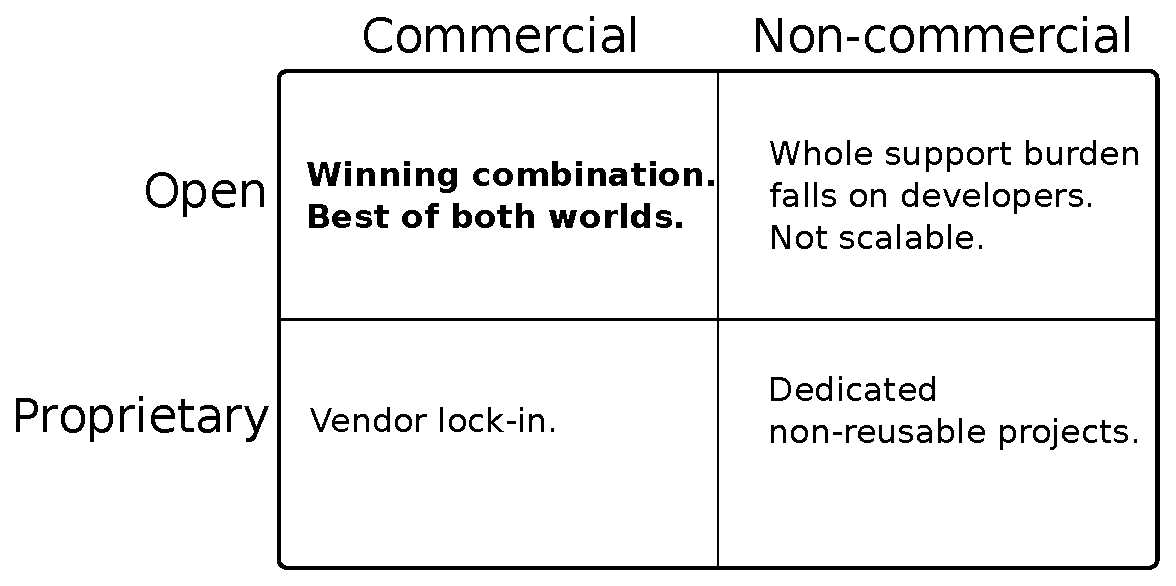
\includegraphics[width=\textwidth]{../../figures/ohwr/commercial_and_open.pdf}
 \end{center} 
\end{frame}

\begin{frame}{Why we use Open Hardware 1/2}
\pause
	\begin{block}{Get a design just the way we want it}
We specify fully the design.
	\end{block}	
\pause
	\begin{block}{Peer review}
	 Get your design reviewed by experts all around the world, including companies!
	\end{block}
\pause
	%\vspace{0.1cm}
\begin{block}{Design re-use}
  When it's Open, people are more likely to re-use it.
	\end{block}
\pause
	\begin{block}{Healthier relationship with companies}
          No vendor-locked situations. Companies selected solely on the basis of technical excellence, good support and price.
	\end{block}
\end{frame}

\begin{frame}{Why we use Open Hardware 2/2}
\pause
\begin{block}{Dissemination of Knowledge}
 One of CERN's key missions!
\end{block}
\pause
\begin{block}{Spend money where you or your funding agencies want}
 \begin{itemize}
   \item Makes life easier for public institutions
   \item Opens the door to smaller companies with good local support
  \end{itemize}
\end{block}	

\end{frame}



\section[WR Intro]{Introduction to White Rabbit}
\subsection{}

\begin{frame}{White Rabbit: an \emph{extension} of Ethernet}

\begin{columns}[c]
  \column{.47\textwidth}
 

  \begin{itemize}
%    \item Few thousands nodes
    \item Bandwidth: 1 Gbps
    \item Single fiber medium
    \item Up to 10 km links
    \item WR Switch: 18 ports
    \item Allows non-WR Devices
    \item Ethernet features (VLAN) \& protocols (SNMP)
  \end{itemize}

  \column{.6\textwidth}
    \begin{center}
    \includegraphics[width=1.0\textwidth]{../../figures/network/wr_network-ethernet.jpg}
    \end{center}
\end{columns}

\end{frame}

\begin{frame}{White Rabbit: an \emph{extension} of Ethernet}


\begin{columns}[c]
  \column{.47\textwidth}
 
  Two separate services (enhancements to Ethernet) provided by WR:
\begin{enumerate}
\item \color{blue!90}{Synchronization:}
  \begin{itemize}
    \item accuracy\\ better than 1 ns
    \item precision in the tens of ps
\end{itemize}
\item \color{red}{Deterministic, reliable and low-latency Control Data delivery}
\end{enumerate}

  \column{.6\textwidth}
    \begin{center}
    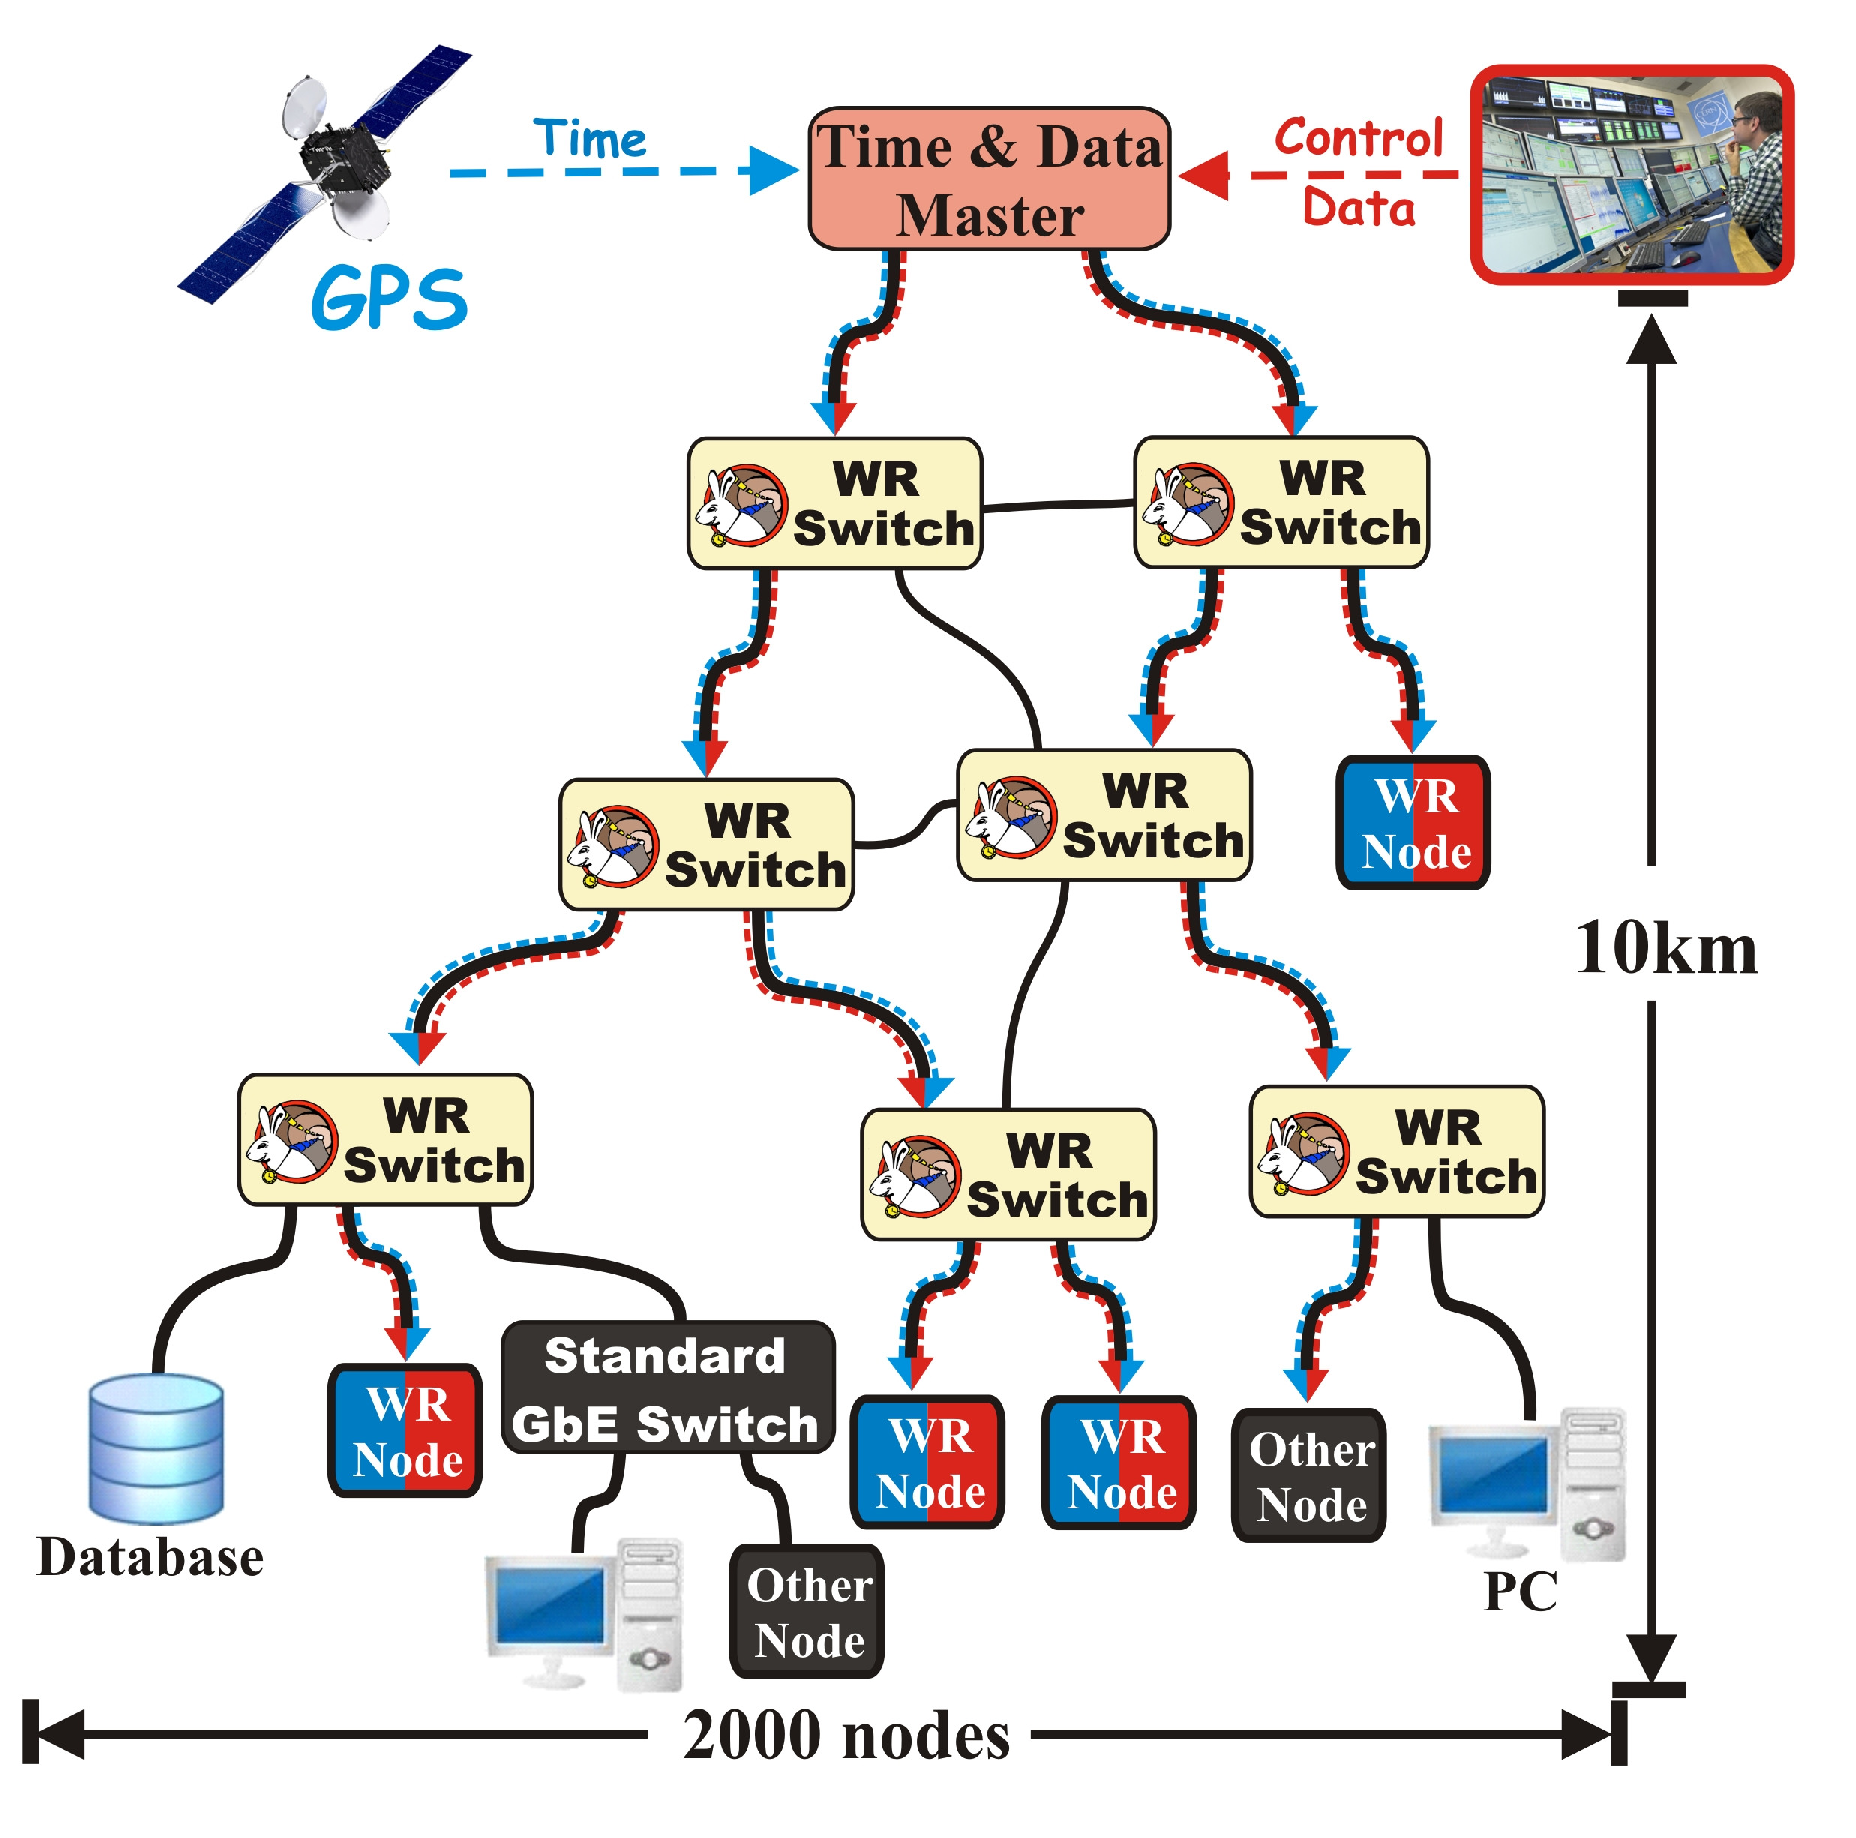
\includegraphics[width=1.0\textwidth]{../../figures/network/wr_network-enhanced_pro.jpg}
    \end{center}
\end{columns}

\end{frame}

\section{Applications}
\subsection{}

\begin{frame}{White Rabbit application examples}
\begin{columns}[c]
  \column{0.65\textwidth}
    \begin{itemize}
      \item Under development:
      \begin{itemize}
	\item \textbf{CERN and GSI}
	\item The Large High Altitude Air Shower Observatory (China)
	\item European deep-sea research infrastructure (KM3NET) 
      \end{itemize}         	
      \item Under evaluation:
      \begin{itemize}
	\item Cherenkov Telescope Array
	\item Long distance Time Transfer
      \end{itemize}         	
    \end{itemize}    
  \column{0.55\textwidth}         
    \begin{center}
      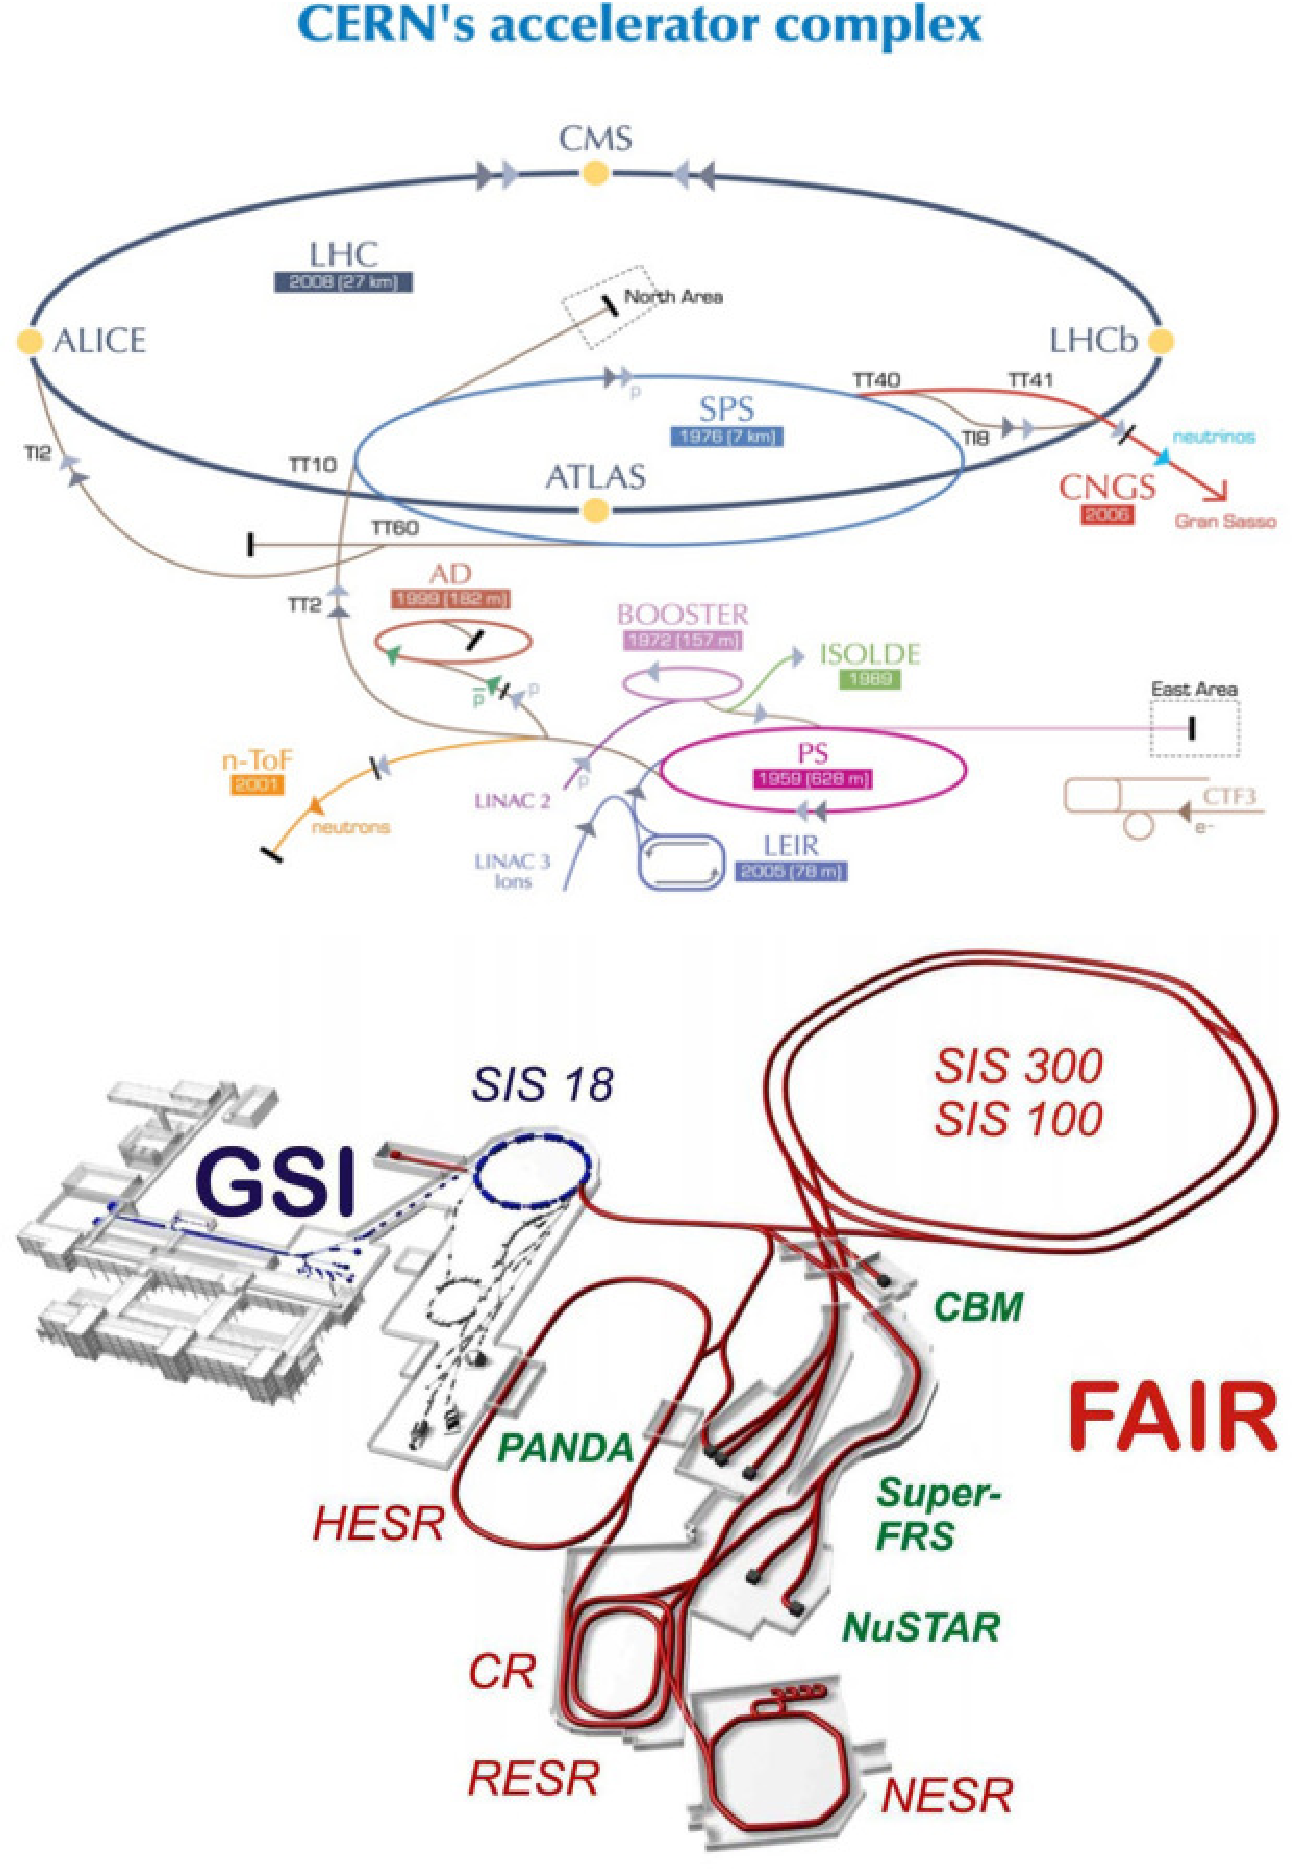
\includegraphics[width=0.6\textwidth]{../../figures/applications/gsiANDcern.pdf}
      \end{center}
  \column{0.6\textwidth}         
\end{columns}
\end{frame}

\begin{frame}{White Rabbit application examples}
\begin{columns}[c]
  \column{0.65\textwidth}
    \begin{itemize}
      \item Under development:
      \begin{itemize}
	\item CERN and GSI
	\item \textbf{The Large High Altitude Air Shower Observatory (China)}
	\item European deep-sea research infrastructure (KM3NET) 
      \end{itemize}         	
      \item Under evaluation:
      \begin{itemize}
	\item Cherenkov Telescope Array
	\item Long distance Time Transfer
      \end{itemize}         	
    \end{itemize}    
  \column{0.55\textwidth}         
    \begin{center}
      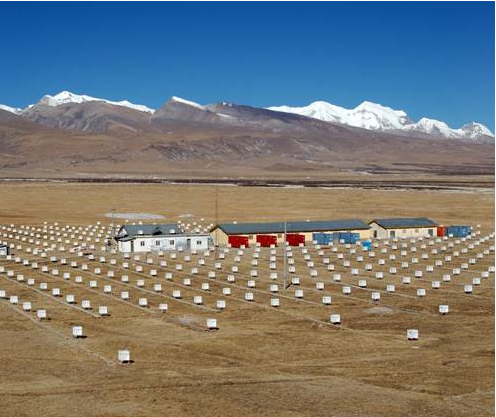
\includegraphics[width=0.6\textwidth]{../../figures/applications/lhaaso.pdf}
      \end{center}
  \column{0.6\textwidth}         
\end{columns}
\end{frame}

\begin{frame}{White Rabbit application examples}
\begin{columns}[c]
  \column{0.65\textwidth}
    \begin{itemize}
      \item Under development:
      \begin{itemize}
	\item CERN and GSI
	\item The Large High Altitude Air Shower Observatory (China)
	\item \textbf{European deep-sea research infrastructure (KM3NET)} 
      \end{itemize}         	
      \item Under evaluation:
      \begin{itemize}
	\item Cherenkov Telescope Array
	\item Long distance Time Transfer
      \end{itemize}         	
    \end{itemize}    
  \column{0.55\textwidth}         
    \begin{center}
      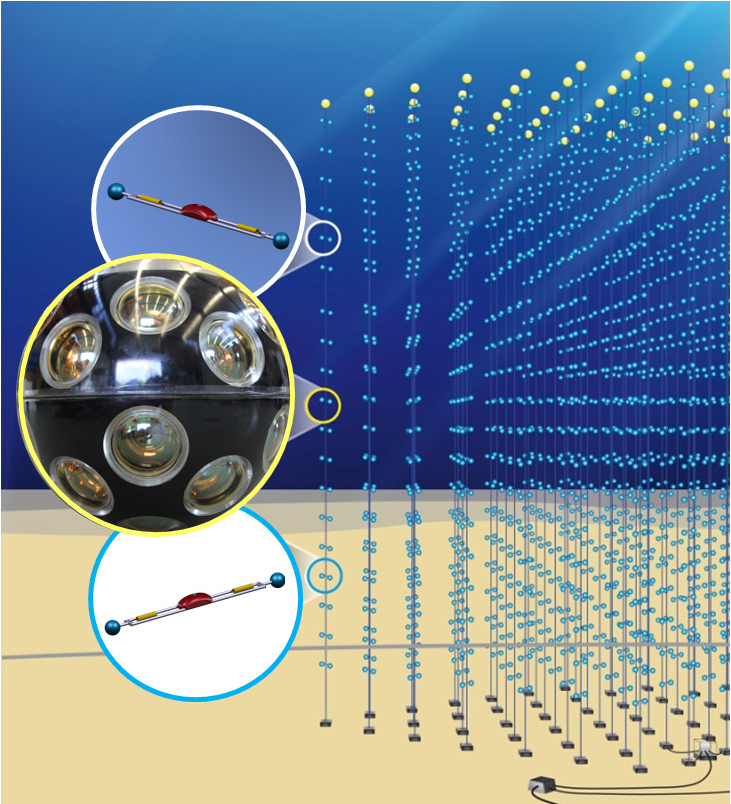
\includegraphics[width=0.6\textwidth]{../../figures/applications/KM3NeT.pdf}
      \end{center}
  \column{0.6\textwidth}         
\end{columns}
\end{frame}

\begin{frame}{White Rabbit application examples}
\begin{columns}[c]
  \column{0.65\textwidth}
    \begin{itemize}
      \item Under development:
      \begin{itemize}
	\item CERN and GSI
	\item The Large High Altitude Air Shower Observatory (China)
	\item European deep-sea research infrastructure (KM3NET) 
      \end{itemize}         	
      \item Under evaluation:
      \begin{itemize}
	\item \textbf{Cherenkov Telescope Array}
	\item Long distance Time Transfer
      \end{itemize}         	
    \end{itemize}    
  \column{0.55\textwidth}         
    \begin{center}
      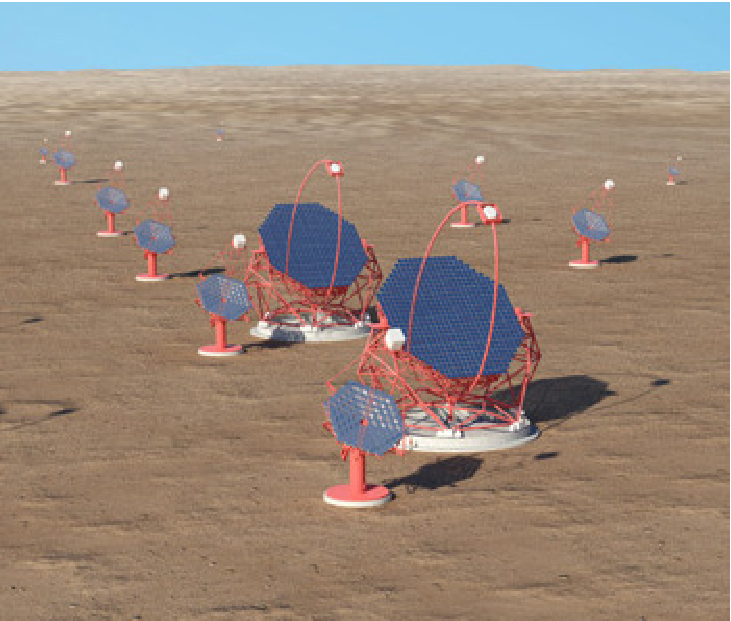
\includegraphics[width=0.6\textwidth]{../../figures/applications/cta.pdf}
      \end{center}
  \column{0.6\textwidth}         
\end{columns}
\end{frame}


\begin{frame}{White Rabbit application examples}
\begin{columns}[c]
  \column{0.65\textwidth}
    \begin{itemize}
      \item Under development:
      \begin{itemize}
	\item CERN and GSI
	\item The Large High Altitude Air Shower Observatory (China)
	\item European deep-sea research infrastructure (KM3NET) 
      \end{itemize}         	
      \item Under evaluation:
      \begin{itemize}
	\item Cherenkov Telescope Array
	\item \textbf{Long distance Time Transfer}
      \end{itemize}         	
    \end{itemize}    
  \column{0.55\textwidth}         
    \begin{center}
      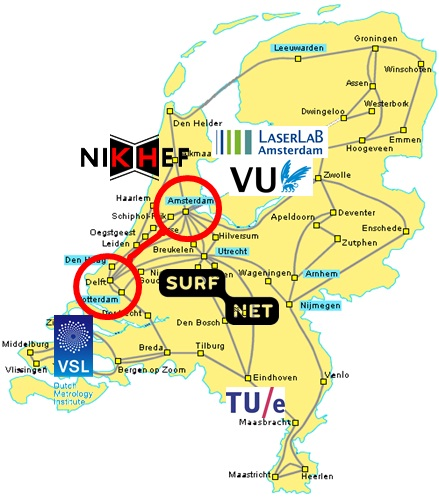
\includegraphics[width=0.6\textwidth]{../../figures/applications/netherlands.jpg}
      \end{center}
  \column{0.6\textwidth}         
\end{columns}
\end{frame}


\begin{frame}{White Rabbit application examples}
\begin{columns}[c]
  \column{0.65\textwidth}
    \begin{itemize}
      \item Under development:
      \begin{itemize}
	\item CERN and GSI
	\item The Large High Altitude Air Shower Observatory (China)
	\item European deep-sea research infrastructure (KM3NET) 
      \end{itemize}         	
      \item Under evaluation:
      \begin{itemize}
	\item Cherenkov Telescope Array
	\item \textbf{Long distance Time Transfer}
      \end{itemize}         	
    \end{itemize}    
  \column{0.55\textwidth}         
    \begin{center}
      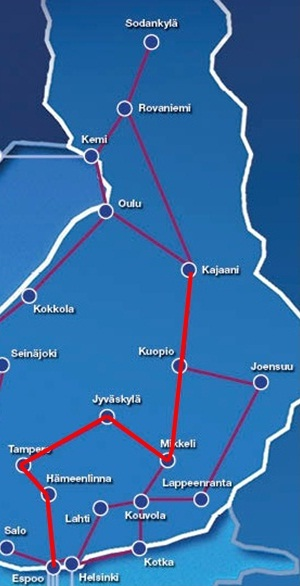
\includegraphics[width=0.6\textwidth]{../../figures/applications/finland.jpg}
      \end{center}
  \column{0.6\textwidth}         
\end{columns}
\end{frame}

\section{Technology}
\subsection{}

\begin{frame}{Precision Time Protocol (IEEE 1588)}

\begin{columns}[c]
  \column{1.5in}
      \begin{center}
	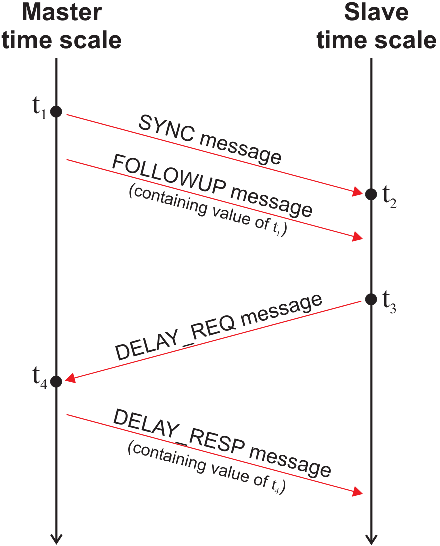
\includegraphics[height=5cm]{../../figures/protocol/ptp_exchange.pdf}
      \end{center}
  \column{2.5in}
      \begin{itemize}
	  \item Frame-based \\ synchronization protocol.
	  \item Synchronizes local clock \\ with the master clock.
	  \item Link delay evaluated by measuring and exchanging
            frames with tx/rx timestamps.
      \end{itemize}
  \end{columns}
\end{frame}

\begin{frame}{Layer 1 Syntonization}

 \begin{block}{Common clock for the entire network}
%    \textbf{Common clock for the entire network}
    \begin{itemize}
	 \item All network devices use the same physical layer clock.
	 \item Clock is encoded in the Ethernet carrier and recovered by the receiver chip.
	 \item Phase detection allows sub-ns delay measurement.
    \end{itemize}
\end{block}

\vspace{-0.2cm}

\begin{center}
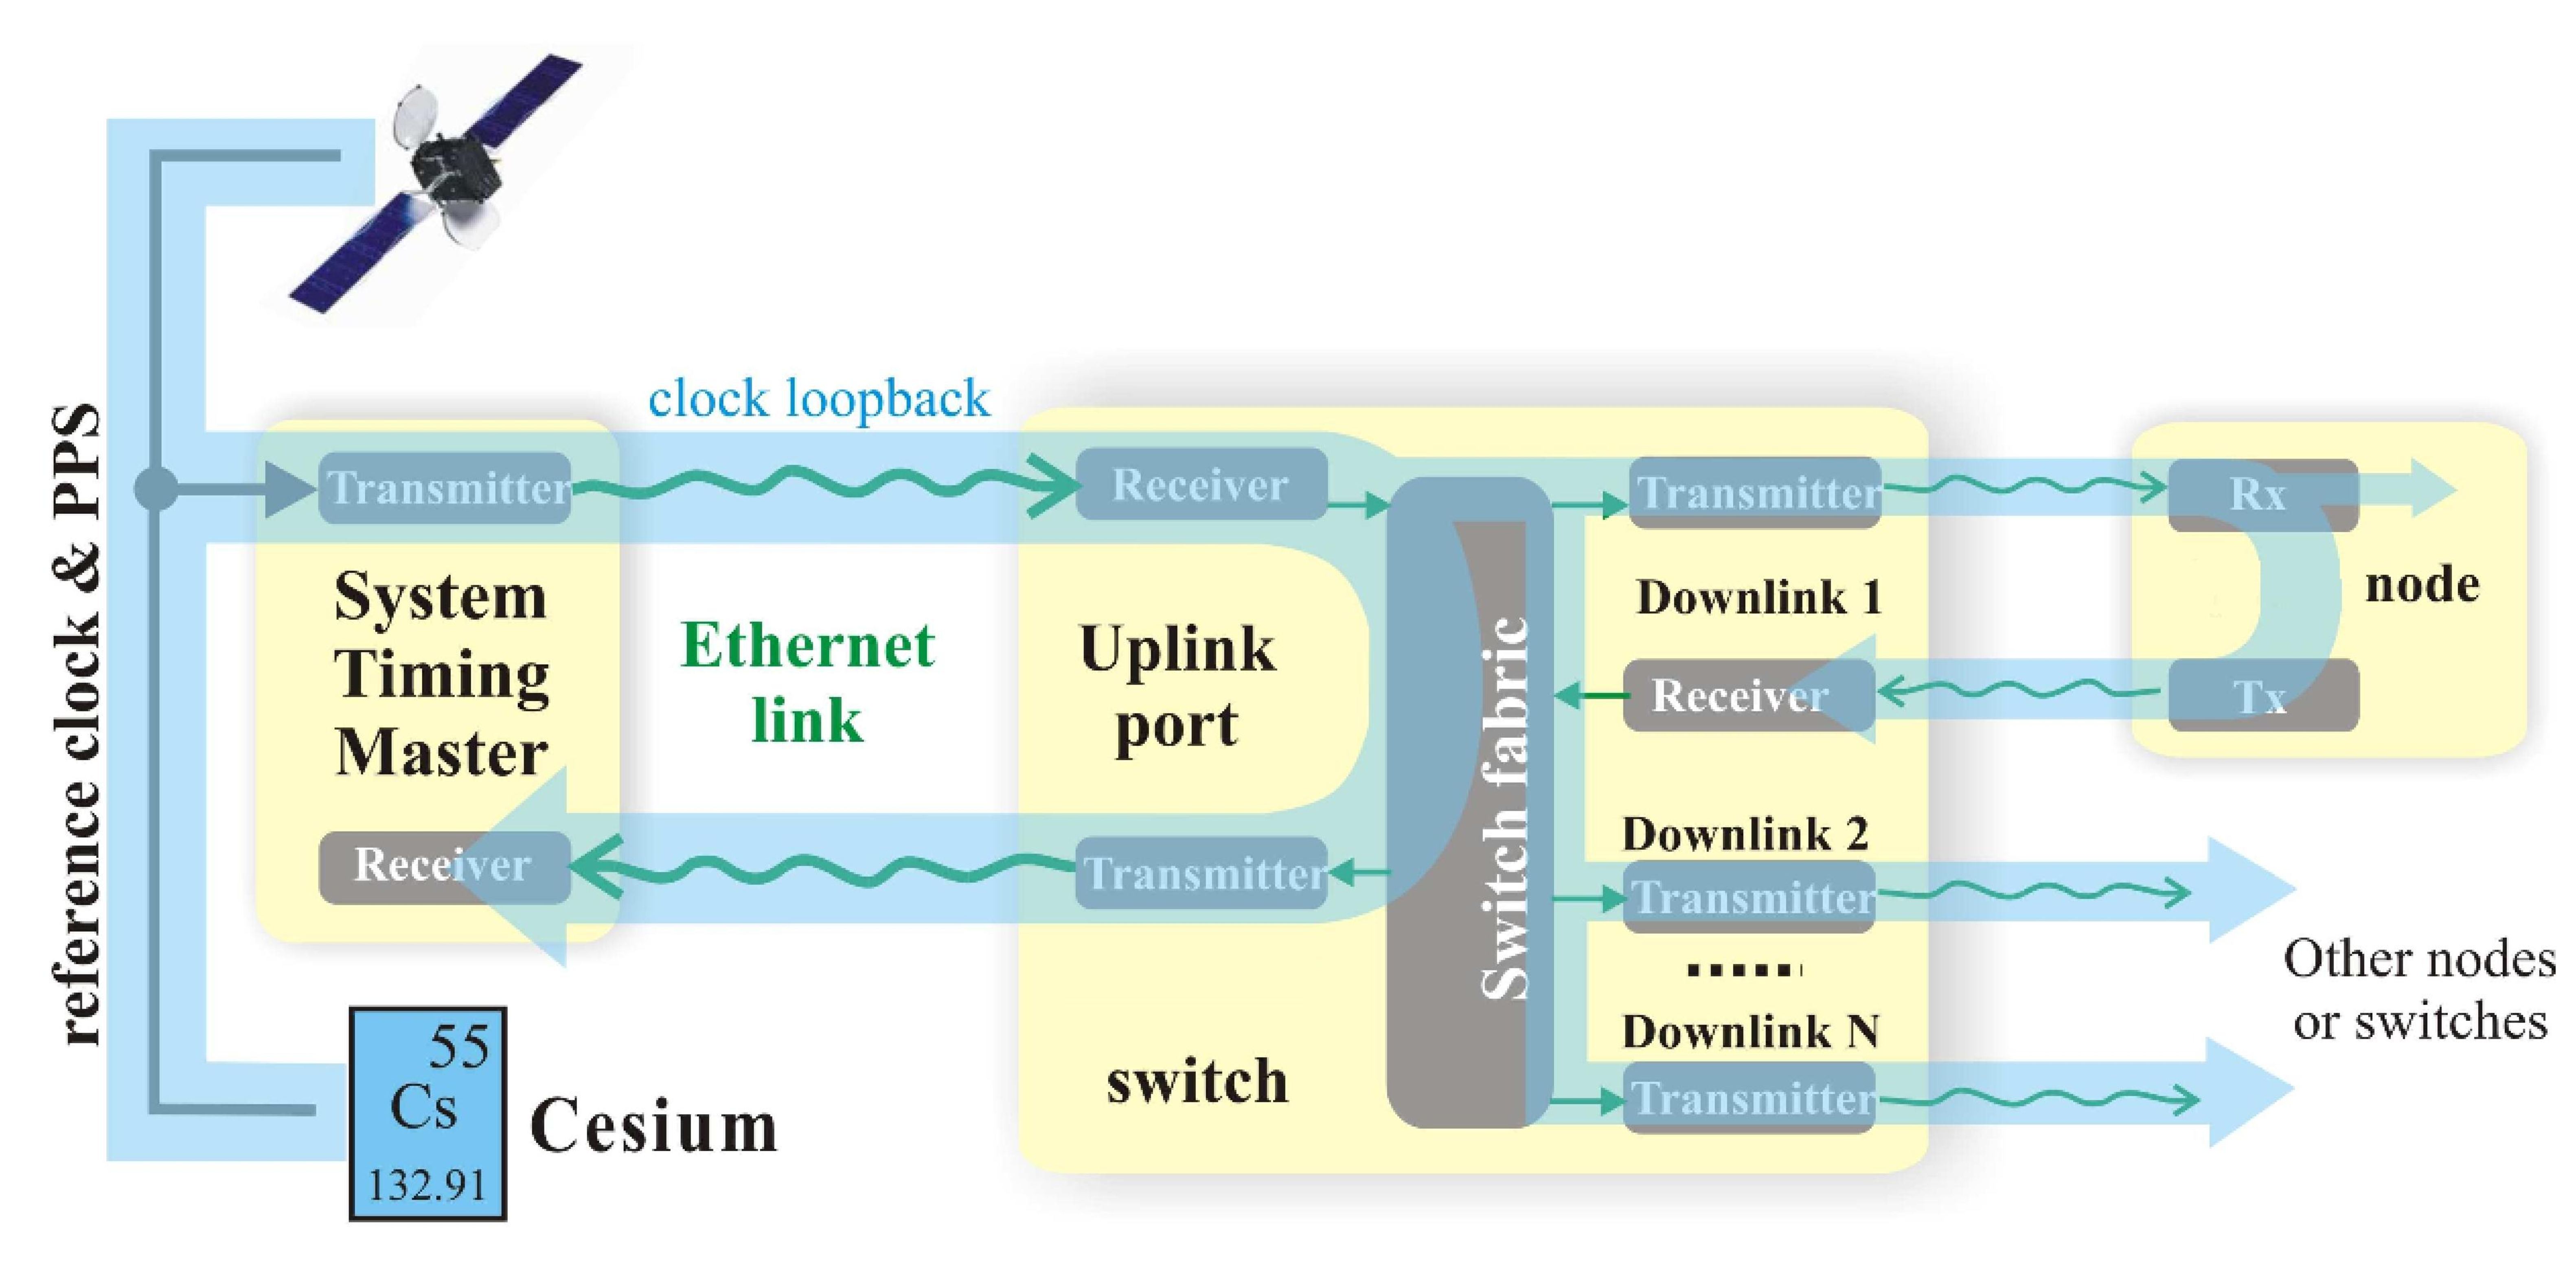
\includegraphics[height=4.5cm]{../../figures/misc/synce_v3.pdf}
\end{center}

\end{frame}

\begin{frame}{Digital Dual Mixer Time Difference}{DDMTD}

\begin{center}
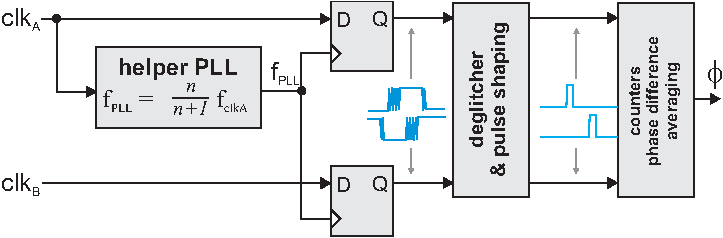
\includegraphics[width=\textwidth]{../../figures/misc/dmtd.pdf}
\end{center}

\end{frame}

\begin{frame}{Link delay model}
 \begin{center}
   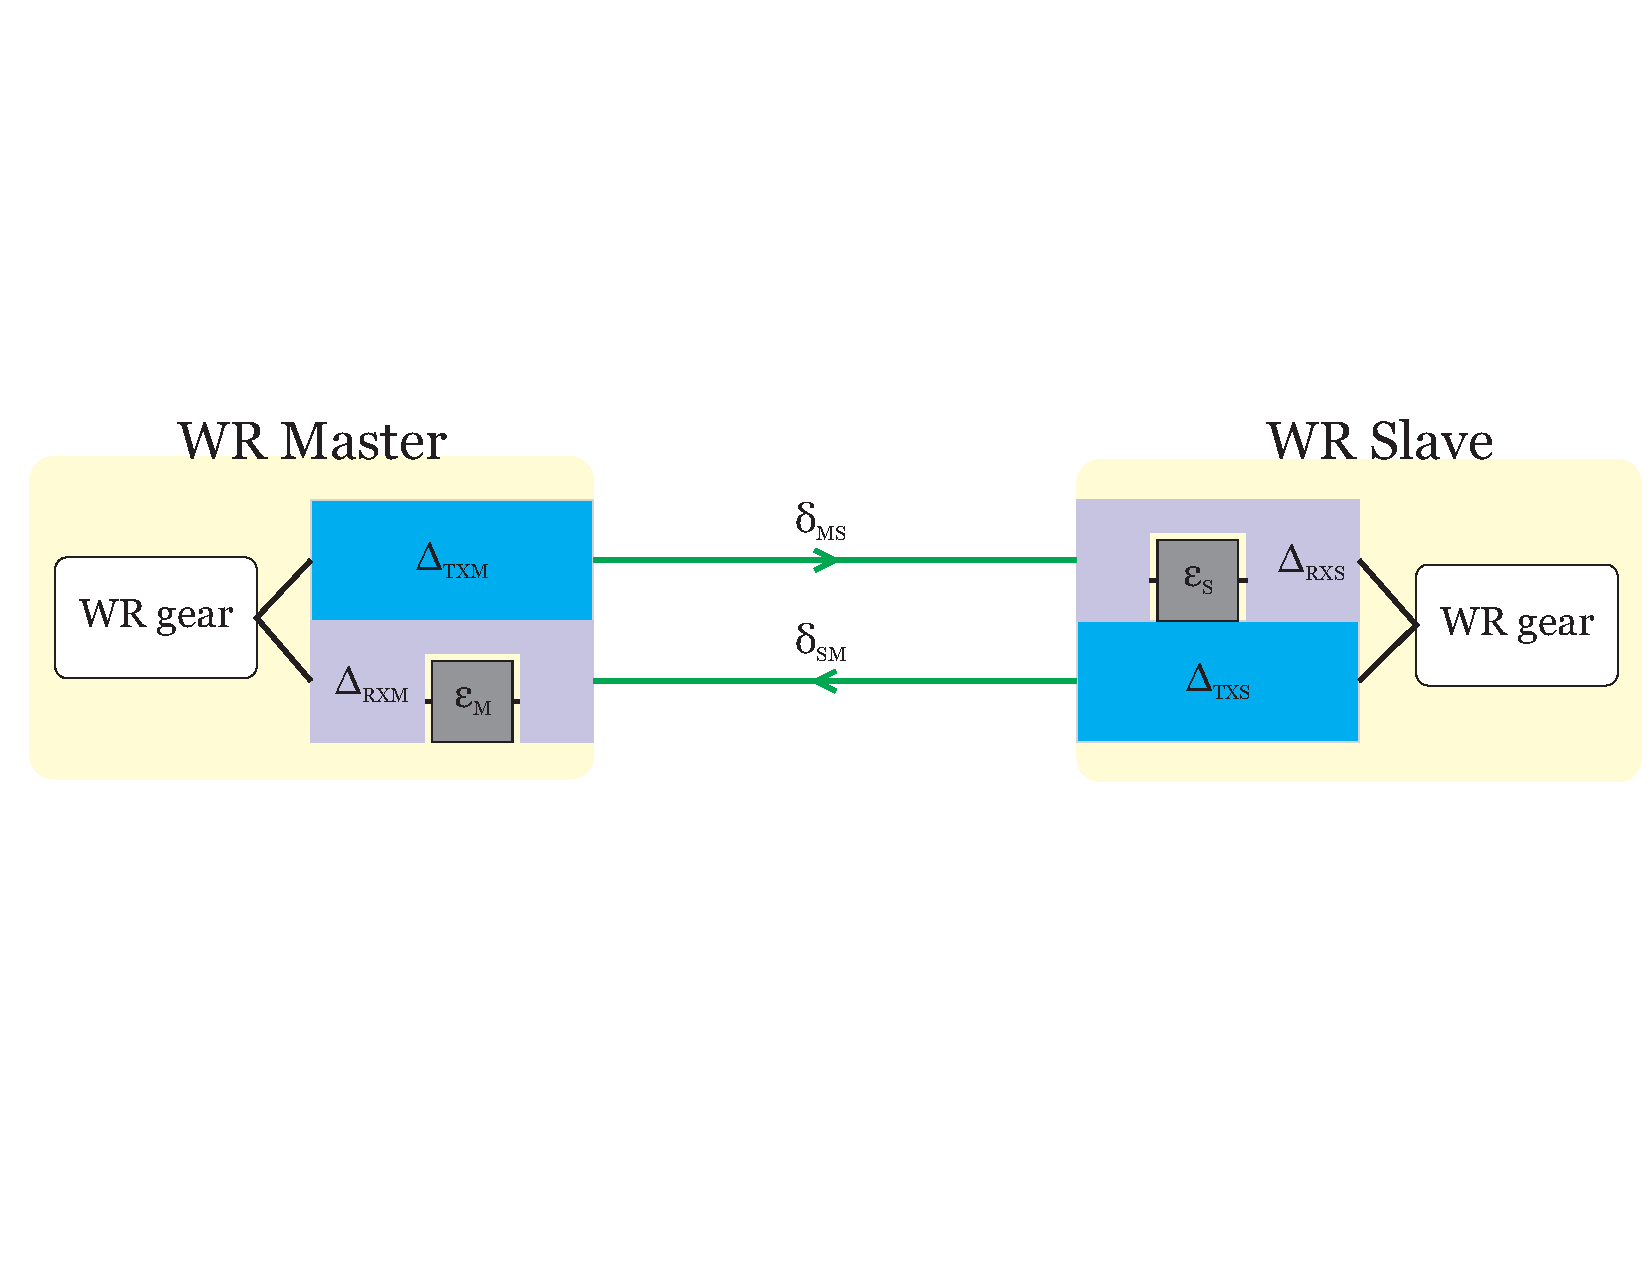
\includegraphics[width=0.9\textwidth]{../../figures/protocol/link-model.pdf}
   \end{center}
\end{frame}

\begin{frame}{White Rabbit Switch}

    \begin{center}
     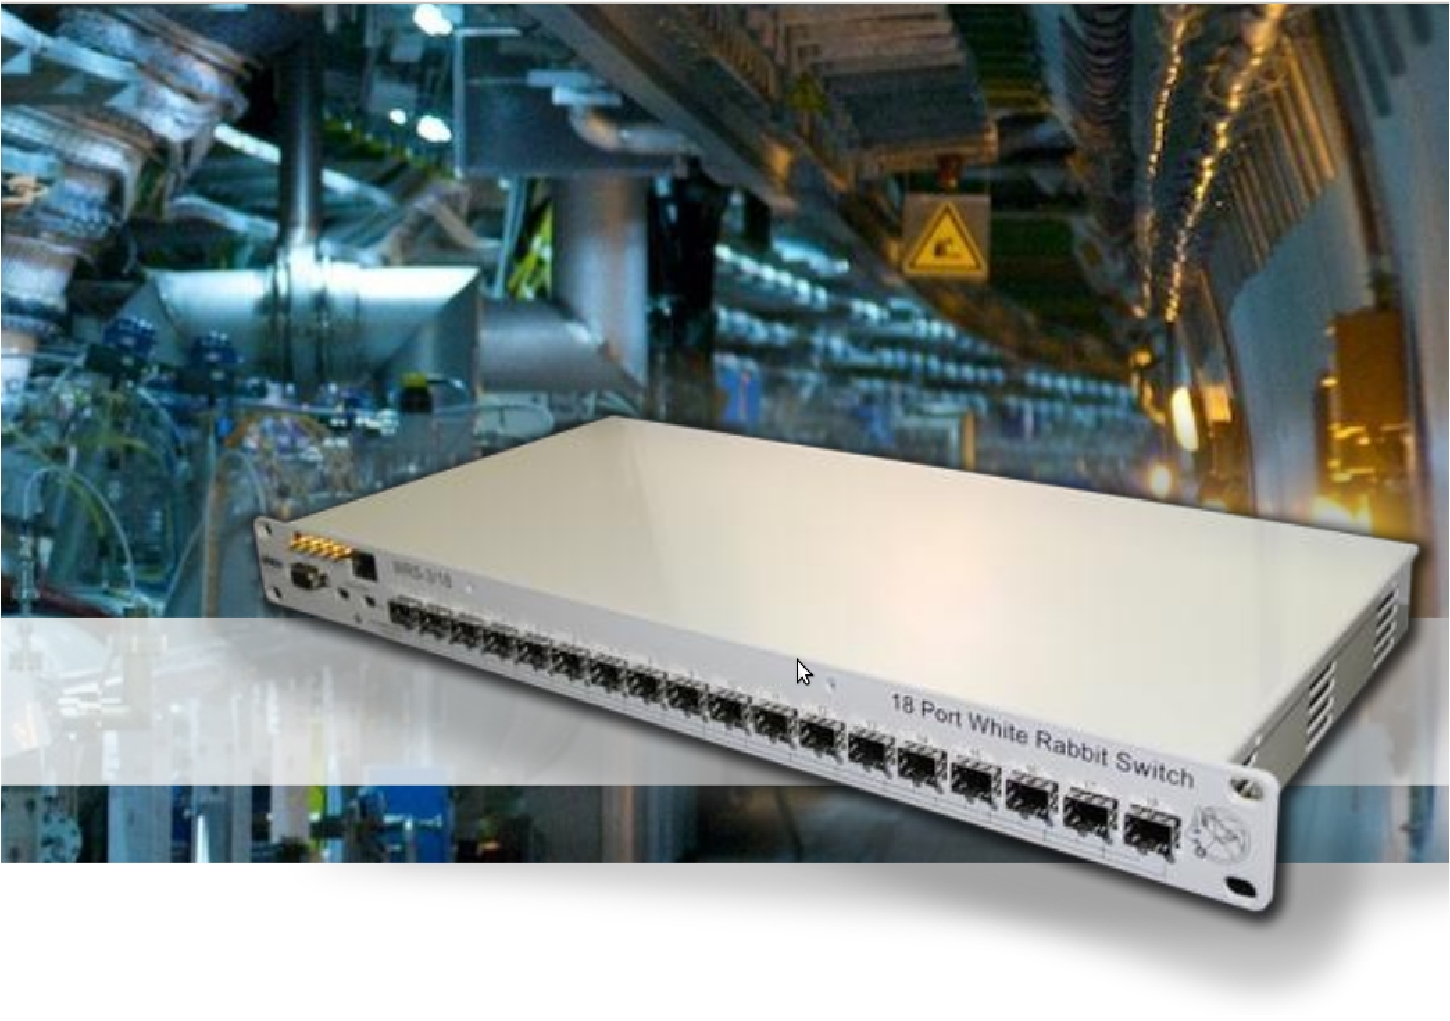
\includegraphics[width=6.0cm]{../../figures/switch/wrSwitchV3.jpg}
    \end{center}
	\begin{itemize}
	\item Central element of WR network
	\item Original design optimized for timing, designed from scratch
	\item 18 1000BASE-BX10 ports
%	\item Capable of driving 10 km of single mode fiber
	\item Open design (H/W and S/W) 
	\item Commercially available
%	\item 200 ps synchronization accuracy
	\end{itemize}
\end{frame}

\begin{frame}{Simplified block diagram of WR switch}
 \begin{center}
   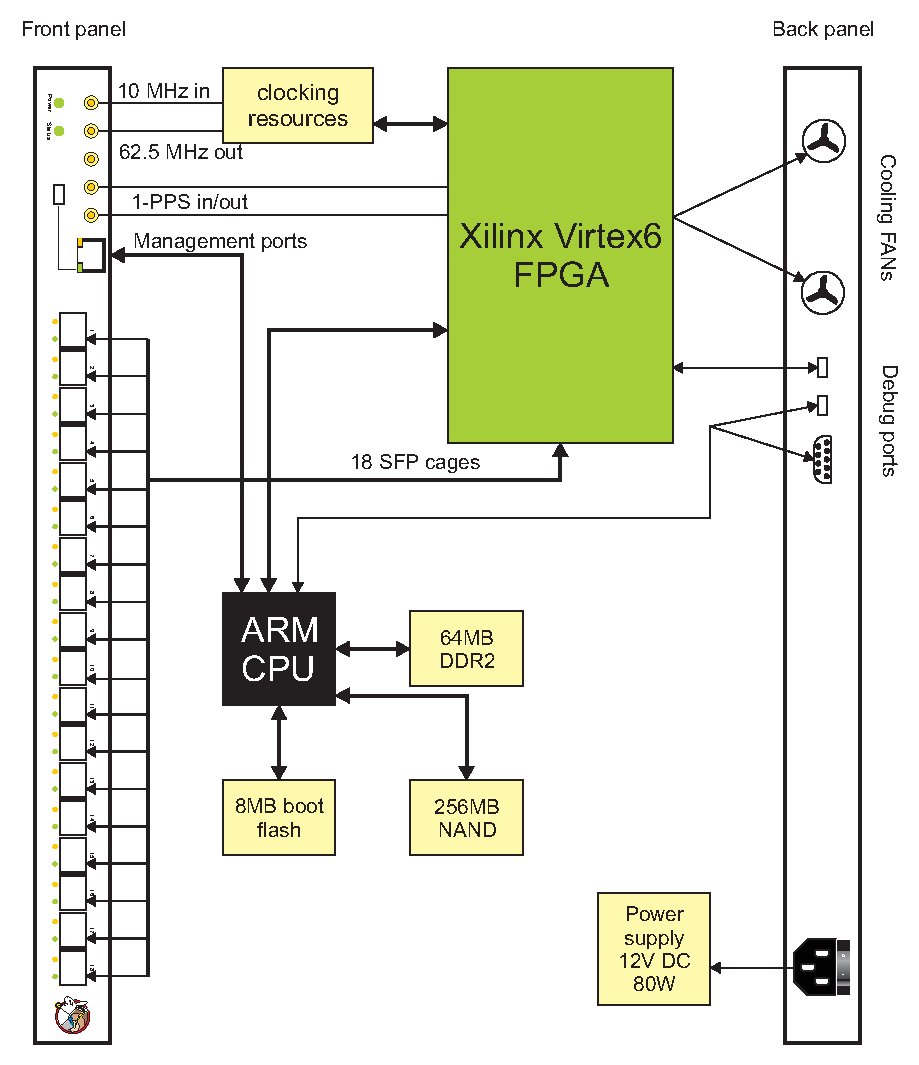
\includegraphics[height=6.9cm]{../../figures/switch/switch_simple_diagram.pdf}
 \end{center} 
\end{frame}


\begin{frame}{WR Node: SPEC board}
    \begin{center}
    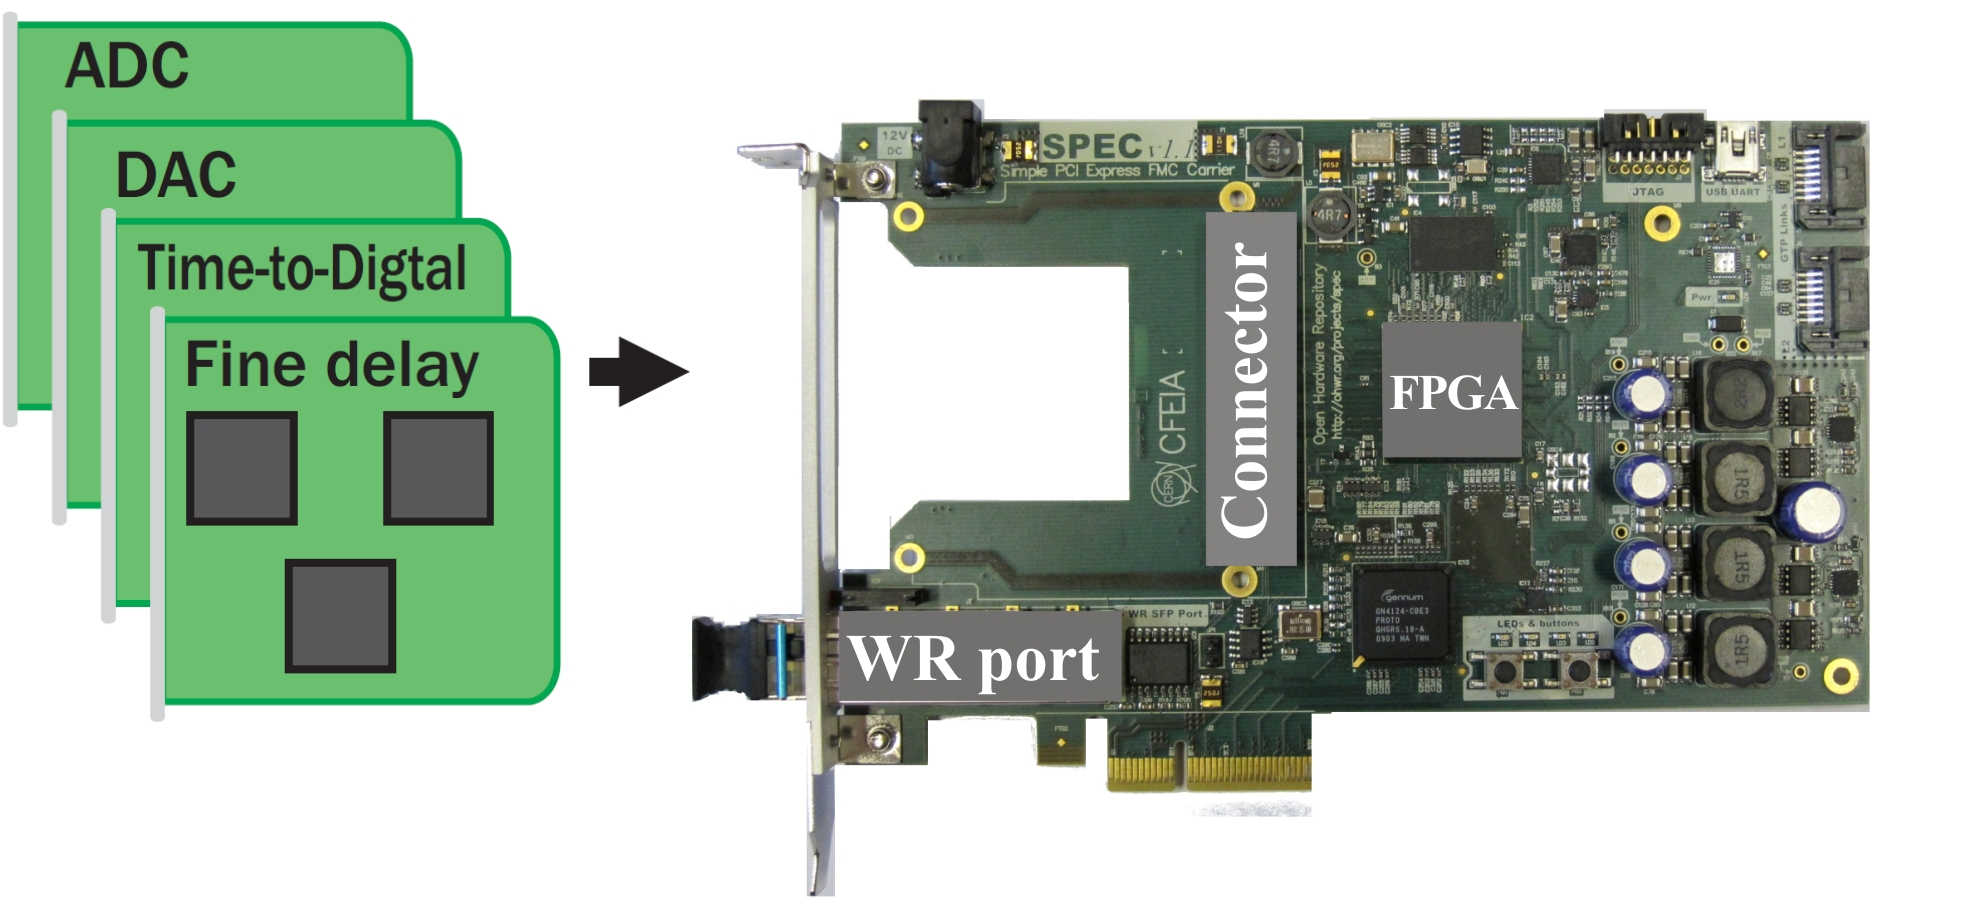
\includegraphics[width=7cm]{../../figures/node/spec.jpg}
    \end{center}

  \begin{columns}[c]
    \column{.01\textwidth}
    \column{.98\textwidth}

	\begin{block}{FMC-based Hardware Kit}
	  \begin{itemize}
%	  \item Carrier boards in PCI-Express, VME, PXIe
	  \item All carrier cards are equipped with a White Rabbit port.
	  \item Mezzanines can use the accurate clock signal and ``TAI''
		\\ (synchronous sampling clock, trigger time tag, ...).
	  \end{itemize}
	\end{block}

    \column{.01\textwidth}
  \end{columns}
\end{frame}

\begin{frame}{White Rabbit PTP Core}
 \begin{center}
   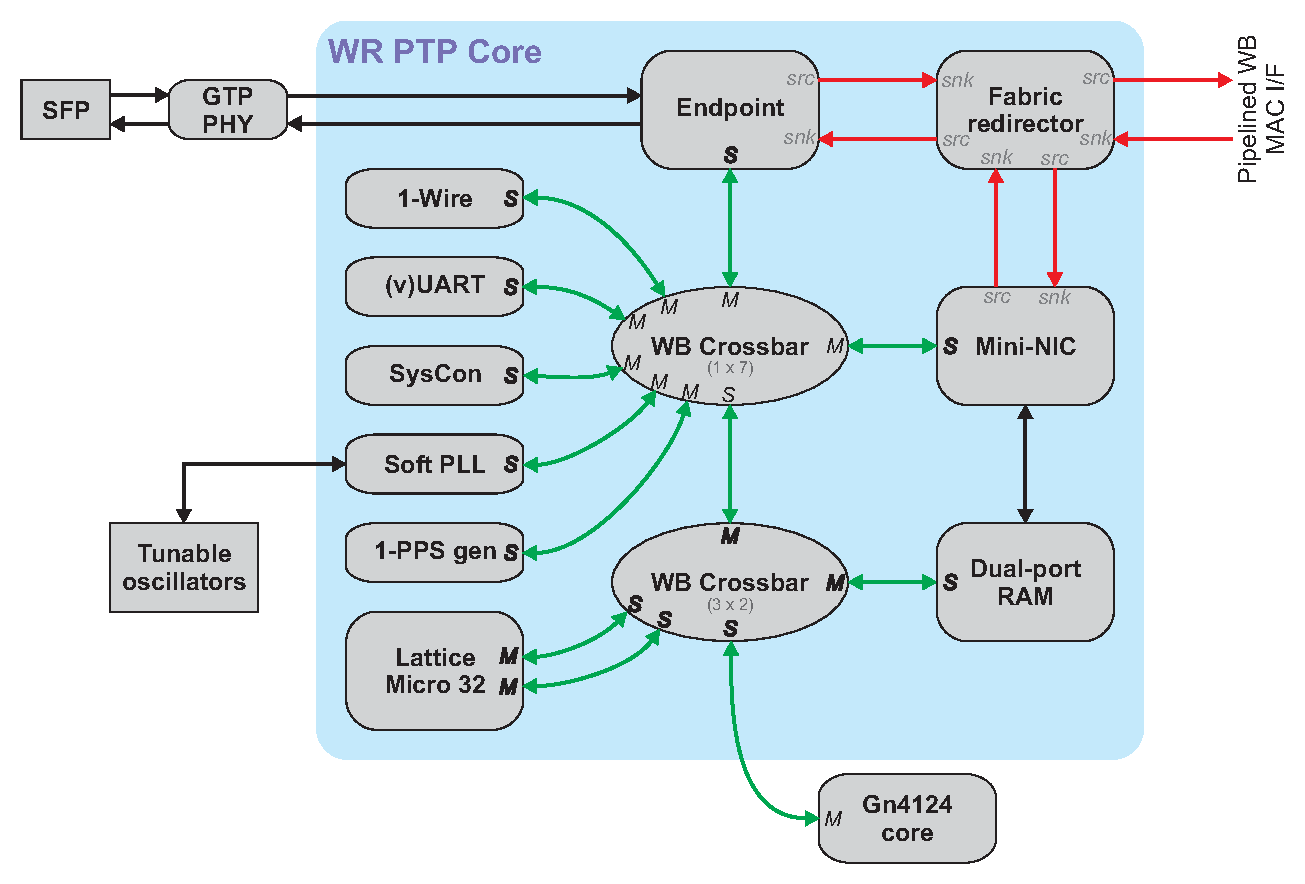
\includegraphics[width=0.9\textwidth]{../../figures/node/wrpc_inside.pdf}
   \end{center}
\end{frame}


\section{Performance}
\subsection{}
\begin{frame}{WR time transfer performance: test setup}

    \begin{center}
    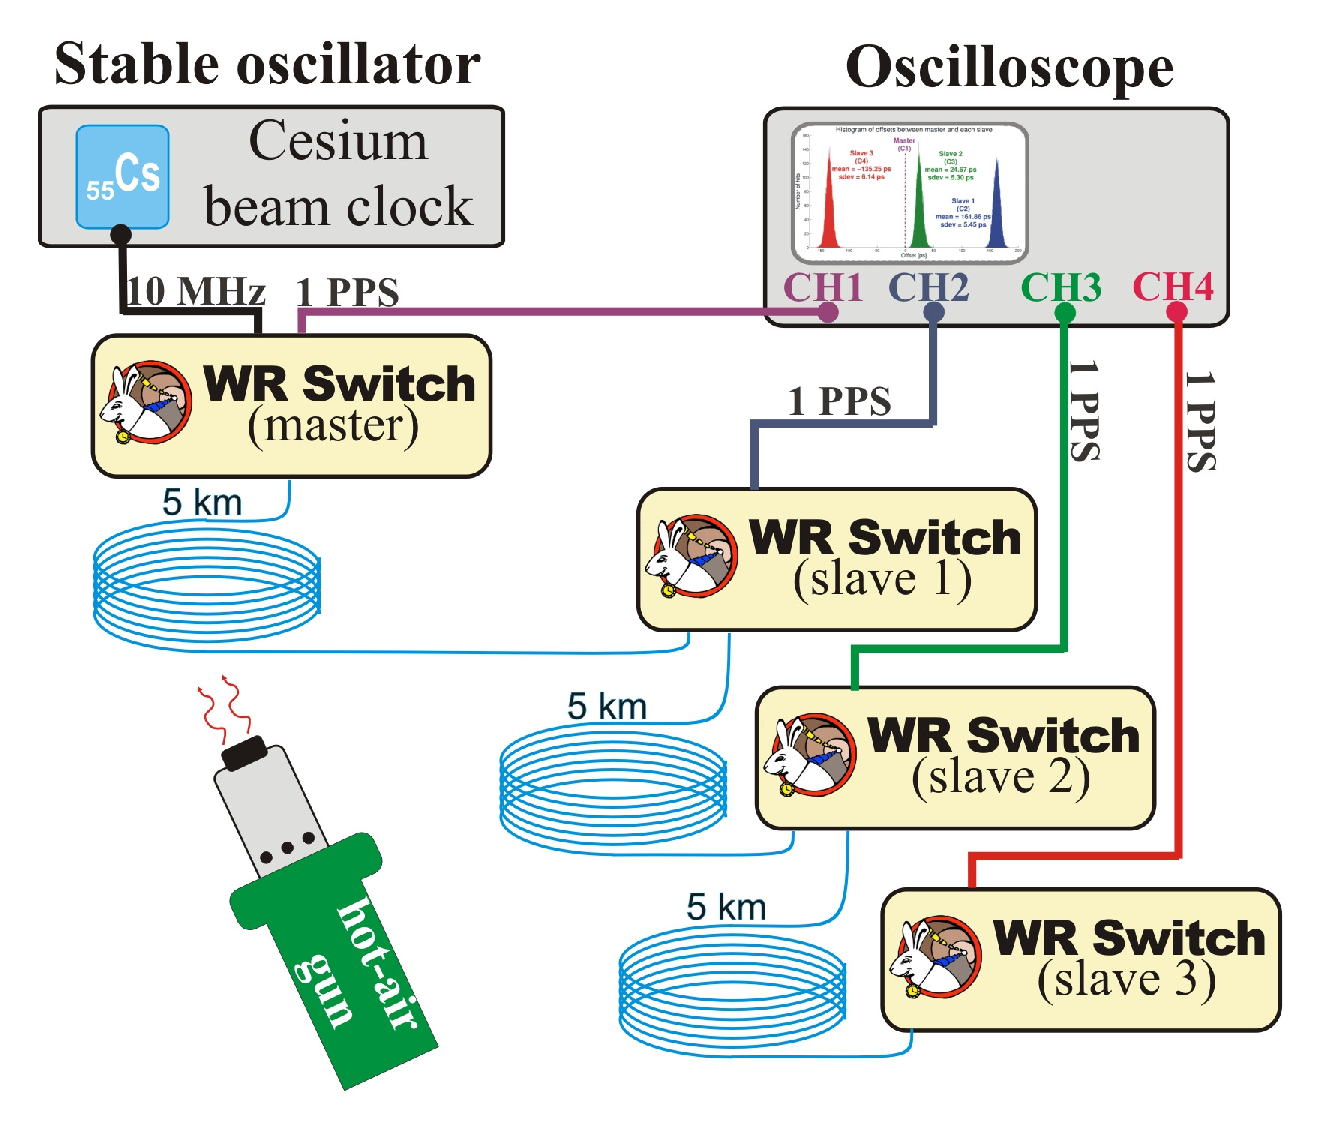
\includegraphics[height=7.0cm]{../../figures/measurements/meas_setup.jpg}
    \end{center}

\end{frame}

\begin{frame}{WR time transfer performance: test results}

    \begin{center}
    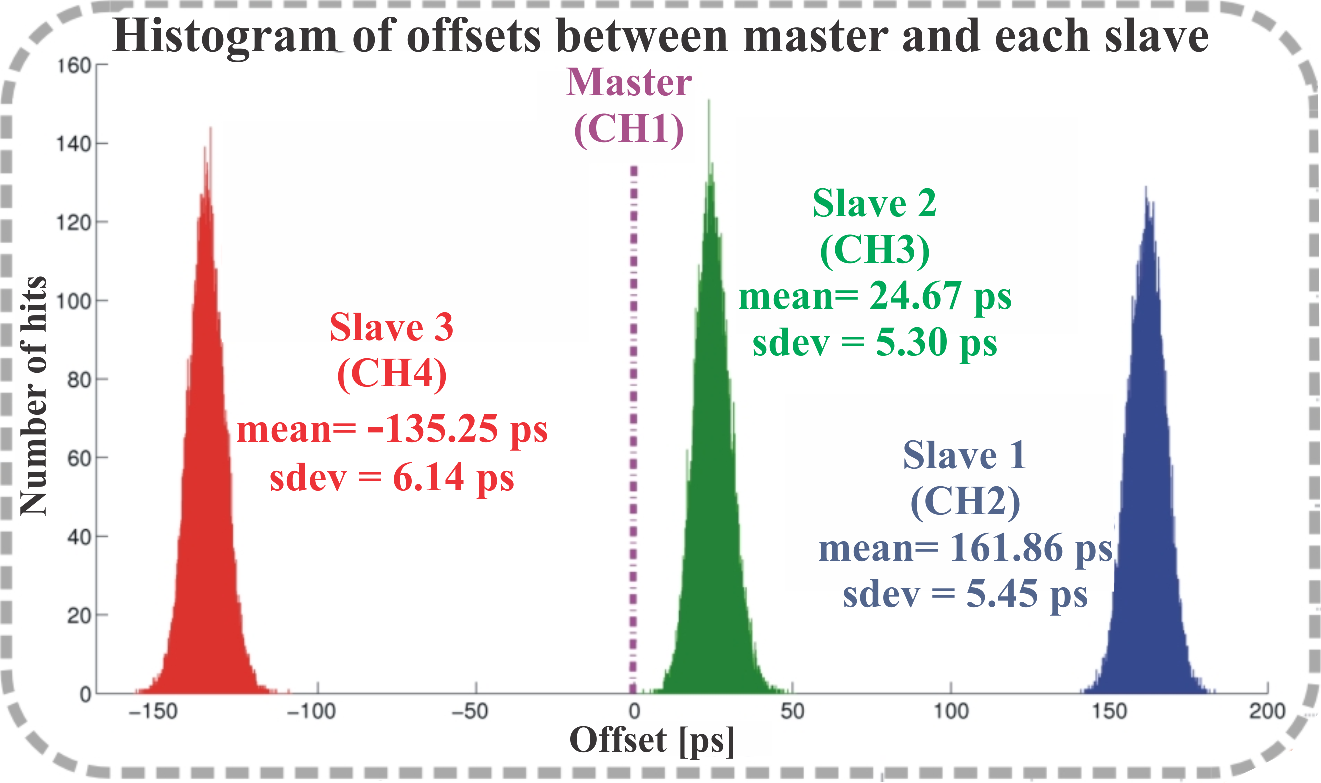
\includegraphics[height=6.0cm]{../../figures/measurements/meas_results.pdf}
    \end{center}

\end{frame}

\begin{frame}{Determinism}
\pause
 \begin{block}{Deterministic by design}
  You know what the frame latency will be because you have the VHDL
  source of the switch FPGA. IEEE 802.1Q headers supported.
 \end{block}
\pause
 \begin{block}{Low latency}
  Cut-through design. Current latency through the switch is
  $\sim$3\textmu s without much effort. Good for (some) feedback systems.
 \end{block}
\pause 
 \begin{block}{Suitable for time-based control and data acquisition}
  Combining a low upper bound in latency and a good common notion of time. 
 \end{block}

\end{frame}

\section{Current developments}
\subsection{}

\begin{frame}{Current developments}
\pause
 \begin{block}{Standardization}
  IEEE 1588 just opened the revision process for the PTP standard,
  which includes an effort on high accuracy. WR is represented in the
  working group.
 \end{block}
\pause
 \begin{block}{Switches and nodes are commercially available}
  Work for the switch now revolves around better diagnostics and
  remote management.
 \end{block}
\pause
 \begin{block}{Robustness}
  Based on redundant information and fast switch-over between
  redundant switches. 
 \end{block}
\end{frame}

\begin{frame}{Ethernet Clock distribution a.k.a. Distributed DDS}
  \begin{center}
    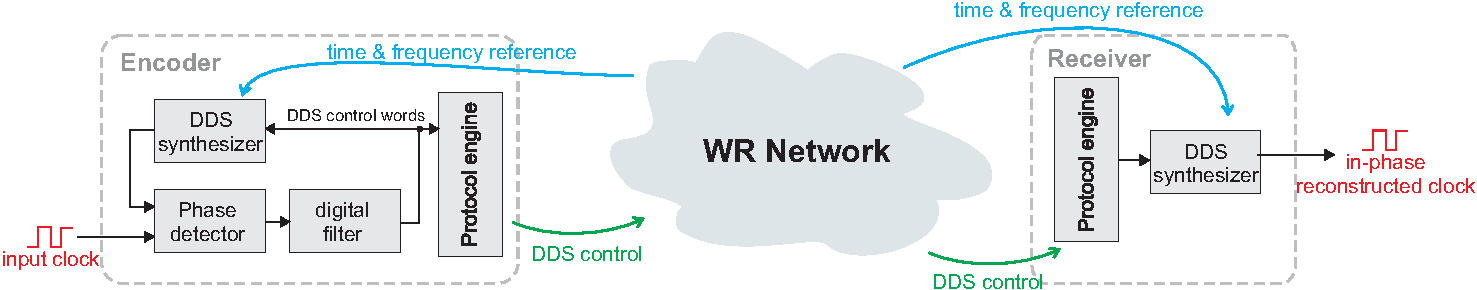
\includegraphics[width=\columnwidth]{../../figures/applications/remote_dds.pdf}
  \end{center}
  \begin{block}{Distributed Direct Digital Synthesis}
    \begin{itemize}
    \item Replaces dozens of cables with a single fiber.
    \item Works over big distances without degrading signal quality.
    \item Can provide various clocks (RF of many rings and linacs)
      with a single, standard link.
    \end{itemize}
  \end{block}
\end{frame}

\begin{frame}{Distributed oscilloscope}
 \begin{center}
   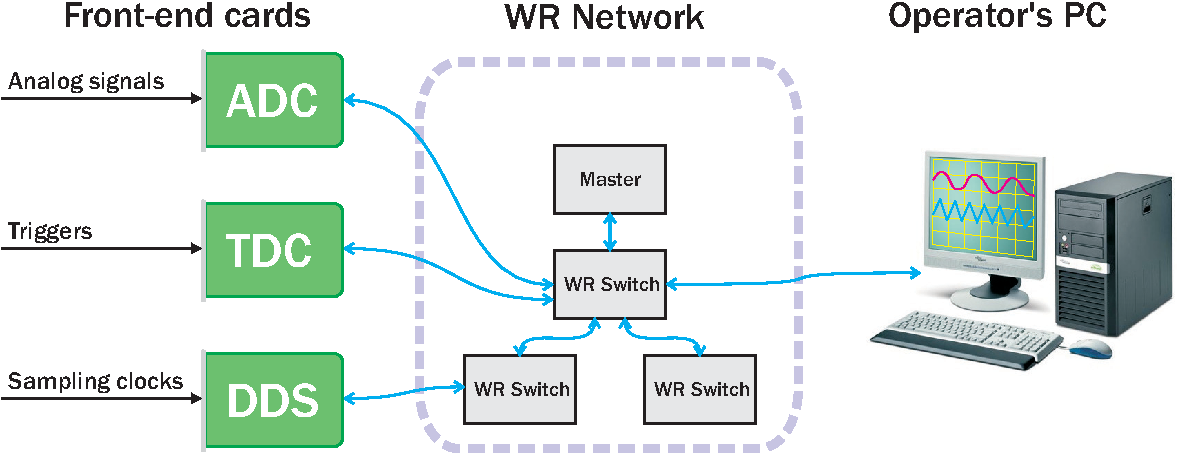
\includegraphics[width=0.9\textwidth]{../../figures/applications/distr_oscill.pdf}
   \end{center}
   \begin{block}{}
     \begin{itemize}
     \item Common clock in entire network: no skew between ADCs.
     \item Ability to sample with different clocks via Distributed DDS.
     \item External triggers can be time tagged with a TDC and used to reconstruct the original time base in the operator's 
PC.
     \end{itemize}
   \end{block}
\end{frame}

\begin{frame}{Support for redundancy}
 \begin{center}
   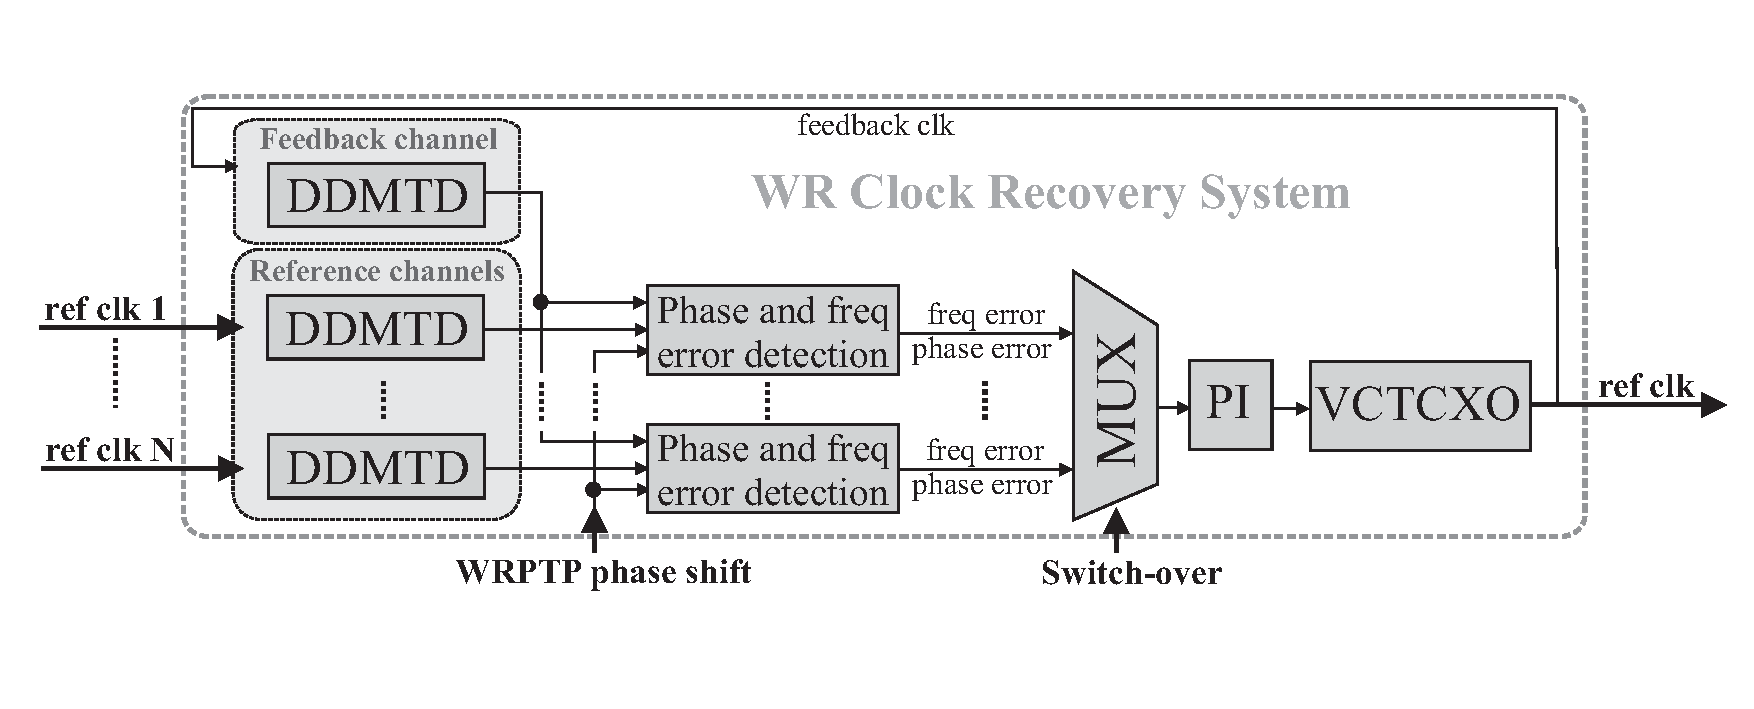
\includegraphics[width=0.9\textwidth]{../../figures/robustness/wrCRS.pdf}
   \end{center}
\end{frame}


\section{Conclusions}
\subsection{}

\begin{frame}{Summary}
 \begin{itemize}
  \pause  
  \item A novel networking technology allowing precise synchronization
    and deterministic data transfer.
  \pause
\item A collaborative distributed effort based on open source hardware
  and software, with an active, enthusiastic community. Everybody is
  welcome to join!  \pause
   \item A versatile working solution for general control and data
    acquisition systems.
 \end{itemize}
 \pause
For more information see http://www.ohwr.org/projects/white-rabbit/wiki
\end{frame}

\end{document}
